\chapter{Il progetto LHC}
\label{cap:PrimoCapitolo}

\sloppy

Lo studio dei prodotti di collisione ad elevata energia negli acceleratori di particelle è di primaria importanza nella fisica delle interazioni fondamentali in quanto permette di scoprire la natura ed il comportamento delle particelle che formano l'universo. In questo capitolo sarà presentato l'acceleratore di particelle LHC e in particolare ci si concentrerà sull'esperimento multifunzionale CMS che ha lo scopo di rilevare muoni generati dalla collisione di protoni ad elevata energia. In questo studio verranno studiati i segnali derivanti dalle camere muoniche, in particolare dalla \textit{regione di barrel} di CMS, ovvero dalla zona centrale dell'esperimento, descrivendo il funzionamento dei rilevatori presenti. Saranno anche discussi brevemente i rilevatori nella \textit{regione di overlap} e nella \textit{regione di endcap} di CMS. \newline
Verrà inoltre studiato nel dettaglio il sistema di Trigger muonico, che ha la funzione di filtrare i segnali provenienti dalle camere muoniche al fine di mantenere solamente gli eventi interessanti, mentre non verrà discusso del sistema di Trigger adronico, che invece ha lo scopo di selezionare eventi rilevanti nella regione delle camere adroniche.

\section{Il Large Hadron Collider}
\label{sec:LHC}
Formato da un anello di circonferenza pari a 27 km, il Large Hadron Collider (LHC) situato al CERN a Ginevra, Svizzera, è il più grande acceleratore di particelle mai costruito, disegnato con lo scopo di studiare, nella sua configurazione finale, collisioni tra protoni con un energia nominale nel centro di massa $\sqrt{s} = 13.6$ TeV e una luminosità istantanea nominale $\mathcal{L} = 2 \times 10^{34}$ \Lumi. 
\begin{figure}[t]
  \centering
  \begin{minipage}[b]{0.43\textwidth}
      \centering
      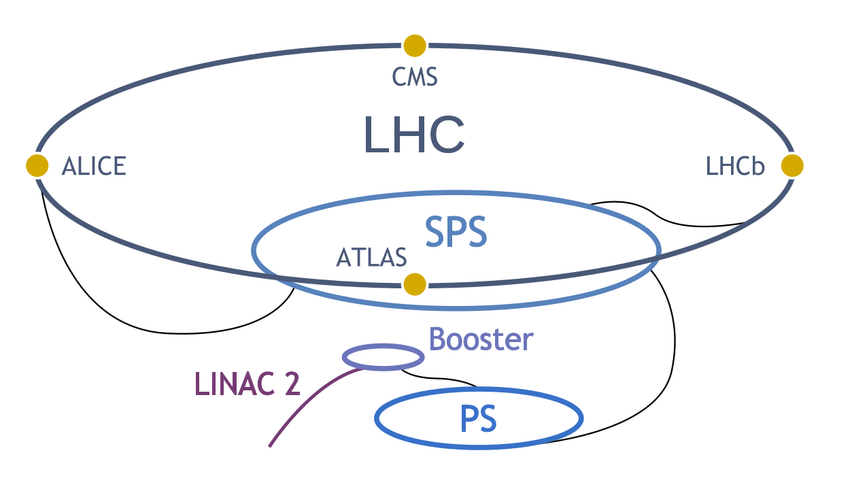
\includegraphics[width=\textwidth]{../ImmaginiTesi/LHC.png} 
  \end{minipage}
  \hfill 
  \begin{minipage}[b]{0.56\textwidth}
      \centering
      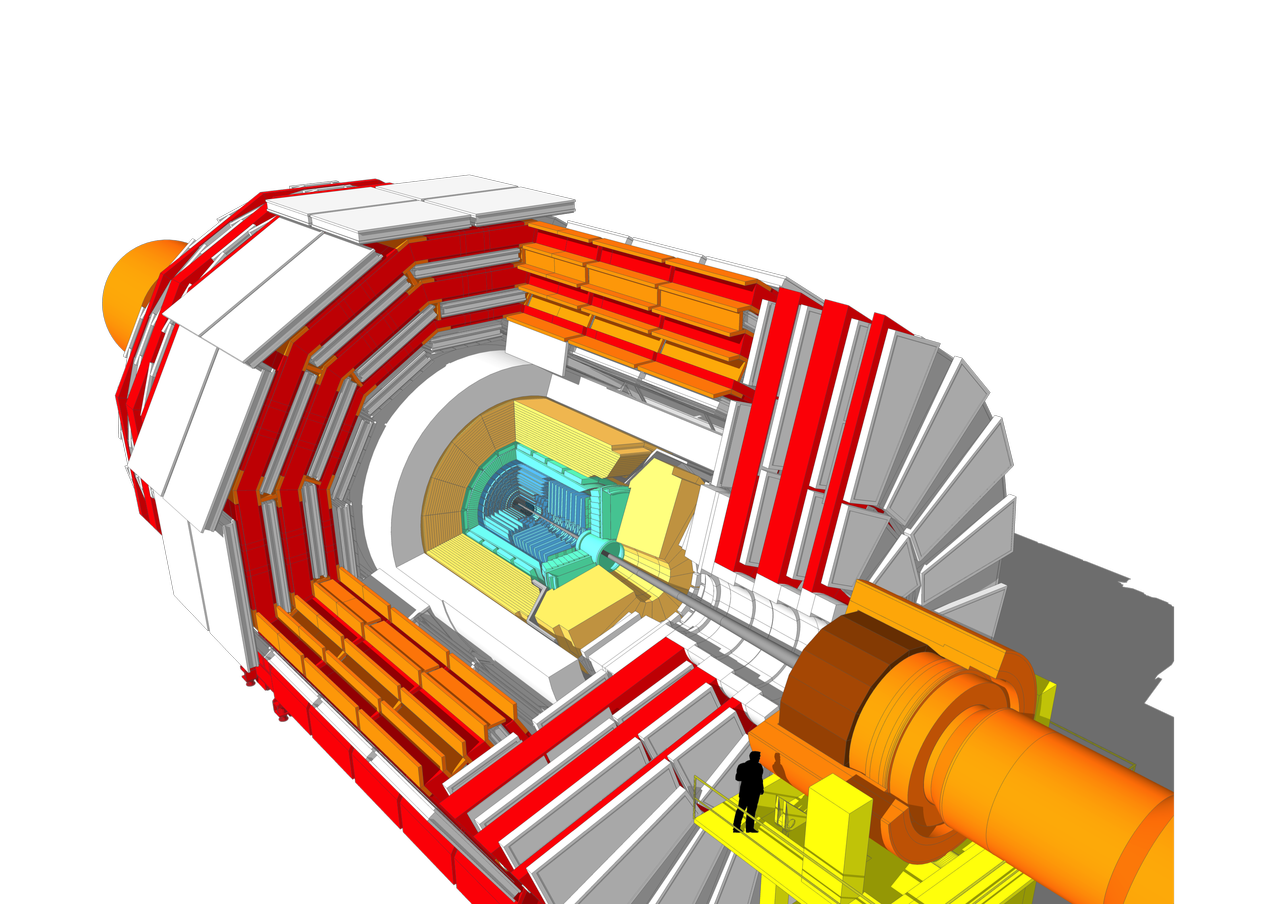
\includegraphics[width=\textwidth]{../ImmaginiTesi/CMS.png} 
  \end{minipage}
  \caption{Struttura dell'LHC e dei suoi rivelatori nei punti di interazione (sinistra), CMS (destra)}
  \label{fig:LHC-CMS}
\end{figure}


Prima di essere immessi in LHC, fasci formati da $1.1 \times 10^{11}$ protoni, subiscono varie fasi di accelerazione, come mostrato in figura \ref{fig:LHC-CMS}: inizialmente ad opera dell' acceleratore lineare Linac, poi dal Proton Synchrotron Booster (PSB), quindi dal Proton Synchrotron (PS) e infine dal Super Proton Synchrotron (SPS), dove vengono iniettati in LHC con una energia di 450 GeV. Circolando in due condotti differenti in direzioni opposte, i protoni vengono accelerati fino a 7 TeV collidendo frontalmente nei punti di interazione, (IP), con una energia nel centro di massa $\sqrt{s} \approx 14$ TeV. L'intervallo temporale tra le collisioni è una unità di misura standardizzata, chiamata \textit{bunch crossing} (BX) e corrisponde a 25ns, ovvero ad un rate di interazioni pari a 40MHz.\newline
I principali esperimenti di LHC sono ATLAS (IP1), ALICE (IP2), CMS (IP5) e LHCb (IP8), nei rispettivi punti di interazione. \newline
ATLAS e CMS sono i due esperimenti multifunzionali di LHC: molti sono gli ambiti di ricerca, dal verificare nuove teorie alla ricerca di nuove particelle. ALICE si occupa dello studio della collisione di ioni pesanti, specializzandosi nella ricerca di gluon-quark plasma. Infine LHCb
si occupa della fisica dei quark beauty con lo scopo di investigare la violazione della simmetria CP.

L'LHC alterna periodi di attività e di raccolta dati (\textit{Run}) con fasi di arresto in cui vengono effettuate opere di upgrade e di manutenzione generale per migliorare le prestazioni del collisore e dei rivelatori. Tra la Run 1, iniziata nel 2009 e finita nel 2013, e la Run 2, tra 2015 e 2018, il sistema di LHC ha subito un incremento dell'energia di collisione protone protone nel centro di massa da 8 a 14 TeV \cite{sirunyan2020performance}. Anche il sistema di acquisizione dati di CMS ha subito importanti miglioramenti (noti come \textit{Phase 1}) rimpiazzando e potenziando hardware, elettronica e software per gestire il maggiore flusso di dati prodotto dalle collisioni ad alta energia. Tra i miglioramenti della Phase 1 vi è l'introduzione del \textit{Pixel Detector}, che permette una migliore gestione della maggiore luminosità istantanea di LHC \cite{Adam:2748381}. Ulteriori miglioramenti sono stati effettuati al sistema di trigger Level 1, L1T, di cui si discuterà in dettaglio nella Sezione \ref{sec:SistemaDiTrigger}. \newline
E' inoltre in programma a partire dal 2026, a seguito della Run 3, un ulteriore upgrade di LHC che porterà un incremento della luminosità istantanea fino a $5\times 10^{34}$ \Lumi, aumentando il numero di collisioni medio per BX da 50 a 140 \cite{collaboration2021phase}. In contemporanea, al fine di sfruttare appieno l'incremento della luminosità di LHC (noto come \textit{High Luminosity LHC}), è previsto un ulteriore upgrade di CMS, noto come \textit{Phase 2}, in particolare al sistema di detector e quello di Trigger. Più nel dettaglio si discuterà della Phase 2 nelle Sezione \ref{sec:Phase2}

\section{Il Compact Muon Solenoid}  
\label{sec:CMSDescrizione}

Locato nel punto di interazione 5 a Cessy, Francia, CMS è formato da un corpo cilindrico di 15 m di diametro e 21.6 m di lunghezza, per un peso di circa 14'000 tonnellate \cite{cms2008cms}. Essendo un esperimento multifunzionale, vari sono gli ambiti di ricerca del rilevatore nel campo della fisica delle alte energie: dopo la scoperta del bosone di Higgs nel 2012 misurare le sue proprietà, attualmente compatibili con il Modello Standard, è diventato di fondamentale importanza. Ugualmente rilevante è anche la ricerca e lo studio di particelle esotiche con l'intento di esplorare Nuova Fisica oltre il Modello Standard. Al fine di identificare questi eventi rari è necessario un sistema di rilevazione e di trigger molto performante \cite{sirunyan2020performance} e a questo scopo assume un'importanza centrale il nuovo sistema di trigger che verrà implementato nella \textit{Phase 2}, che darà la possibilità di verificare queste teorie ricercando fenomeni esotici.

L'origine del sistema di coordinate del Compact Muon Solenoid è centrato nel punto di collisione nominale dei fasci di protoni. L' asse \textit{y} è verticale, l'asse \textit{x} punta verso il centro di LHC e l'asse \textit{z}, segue la regola della mano destra, verso le montagne del Giura. L'angolo azimutale $\phi$ è misurato nel piano \textit{x-y} e l'angolo polare $\theta$ dall'asse \textit{z}. Sono di comune utilizzo variabili Lorentz invarianti nel contesto di condizioni ultrarelativistiche: per questo motivo la pseudorapidità, definita come $\eta = -\ln\left(\theta/2\right)$, è spesso preferita alla coordinata angolare $\theta$. Per tanto il sistema di coordinate adottato a CMS è il sistema \textit{R-$\eta$-$\phi$} \cite{Quertenmont:2010ota}.

\subsection{I rilevatori di CMS}

Di seguito una panoramica della struttura di CMS, Figura \ref{fig:LHC-CMS}, dalle componenti più interne fino a quelle più esterne \cite{MasterThesisNicLai}:

\begin{itemize}
  \item \textbf{Silicon Strip Tracker (SST):} Esegue una ricostruzione delle tracce e misurazione del momento trasverso di particelle originate da processi di interazione, producendo un segnale elettrico ogni volta che una particella passa attraverso.
  \item \textbf{Electromagnetic Calorimeter (ECAL):} Costruito da pannelli di tungstato di piombo (\si{PbWO_4}), materiale scintillante che facilita processi di \textit{cascata elettromagnetica}, permette di effettuare misure di energia di fotoni ed elettroni.
  \item \textbf{Hadronic Calorimeter (HCAL):} Permette la misurazione delle energie degli adroni grazie al fenomeno della \textit{cascata adronica}, indotta dai materiali di cui è costituito l'HCAL, in particolare acciaio e bronzo. Questa viene rilevata da scintillatori plastici che convertono l'energia rilasciata dagli adroni in segnali luminosi, amplificati da fotomoltiplicatori.
  \item \textbf{Solenoide superconduttore:} Formato dal superconduttore Niobio-Titanio (NbTi), produce un campo magnetico di intensità 3.8T nel nucleo. Un campo magnetico così elevato è fondamentale per permettere la curvatura di particelle cariche prodotte dalle collisioni, la cui rivelazione di tale curvatura permette di risalire a momento e carica delle stesse.
  \item \textbf{Camere muoniche:} Essendo i muoni particelle elementari cariche poco interagenti, il sistema di rilevazione muonico occupa una significativa porzione del volume di rilevatori di CMS. Suddiviso in tre regioni, \textit{barrel}, \textit{overlap} ed \textit{endcap}, il sistema delle camere muoniche copre il piano della pseudorapidità nel range $|\eta| < 2.4$, permettendo la rivelazione delle tracce di muoni usando tre diverse tecnologie: \textit{Drift Tube} (DT), \textit{Resistive Plate Chamber} (RPC) e \textit{Cathode Strip Chamber} (CSC) come mostrato in Figura \ref{fig:SectorEtaView} \cite{TheMuonProject}.
\end{itemize}


\subsubsection{Camere muoniche}

\begin{figure}[t]
  \centering
  \begin{minipage}[b]{0.48\textwidth}
      \centering
      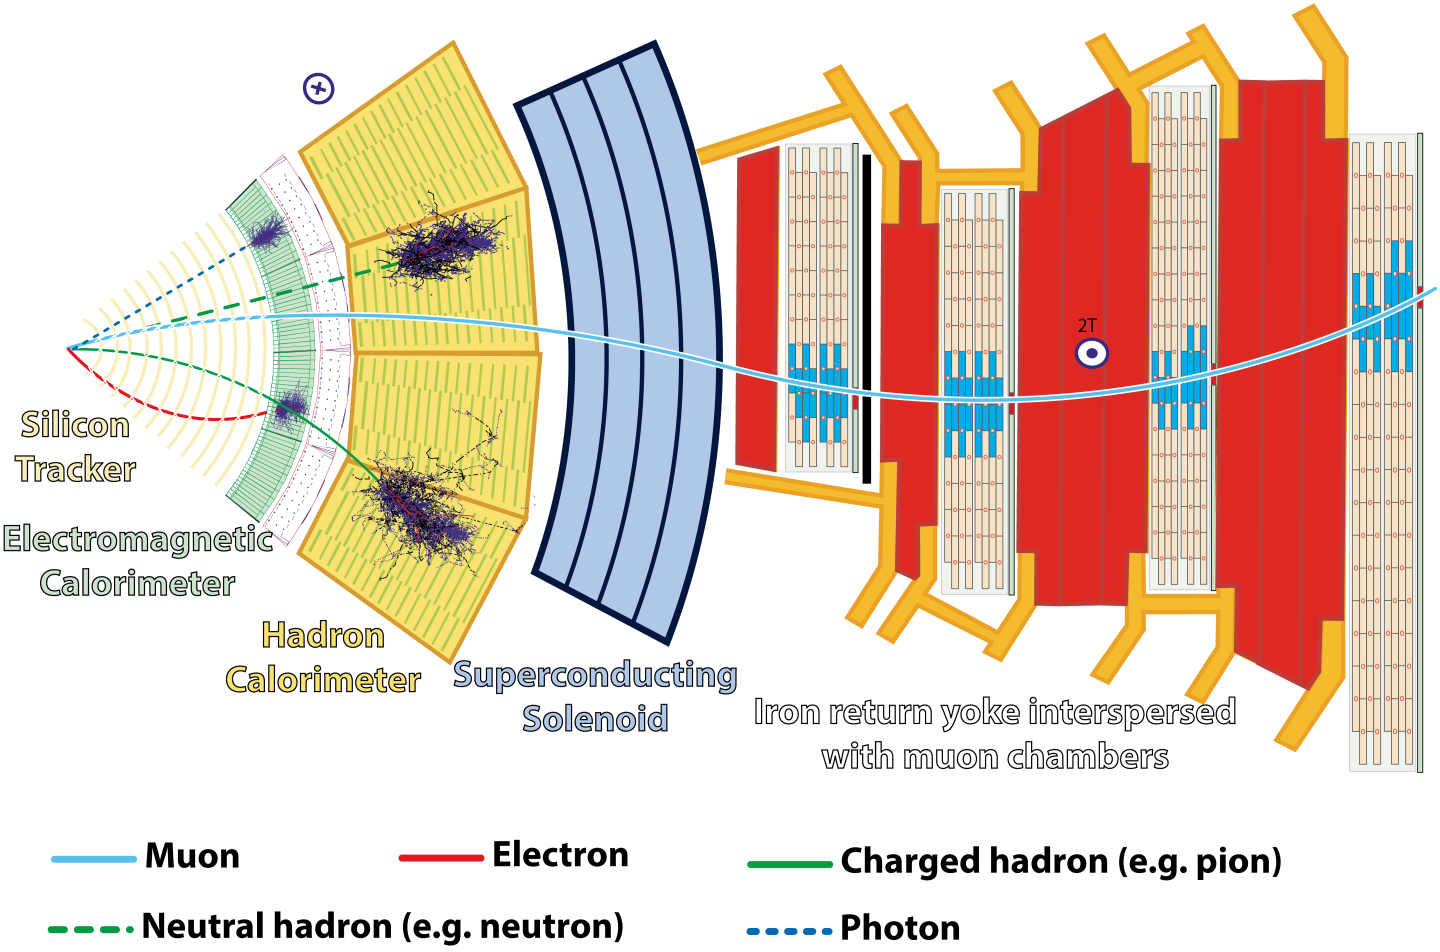
\includegraphics[width=\textwidth]{../ImmaginiTesi/CMS slice.png} 
  \end{minipage}
  \hfill 
  \begin{minipage}[b]{0.48\textwidth}
      \centering
      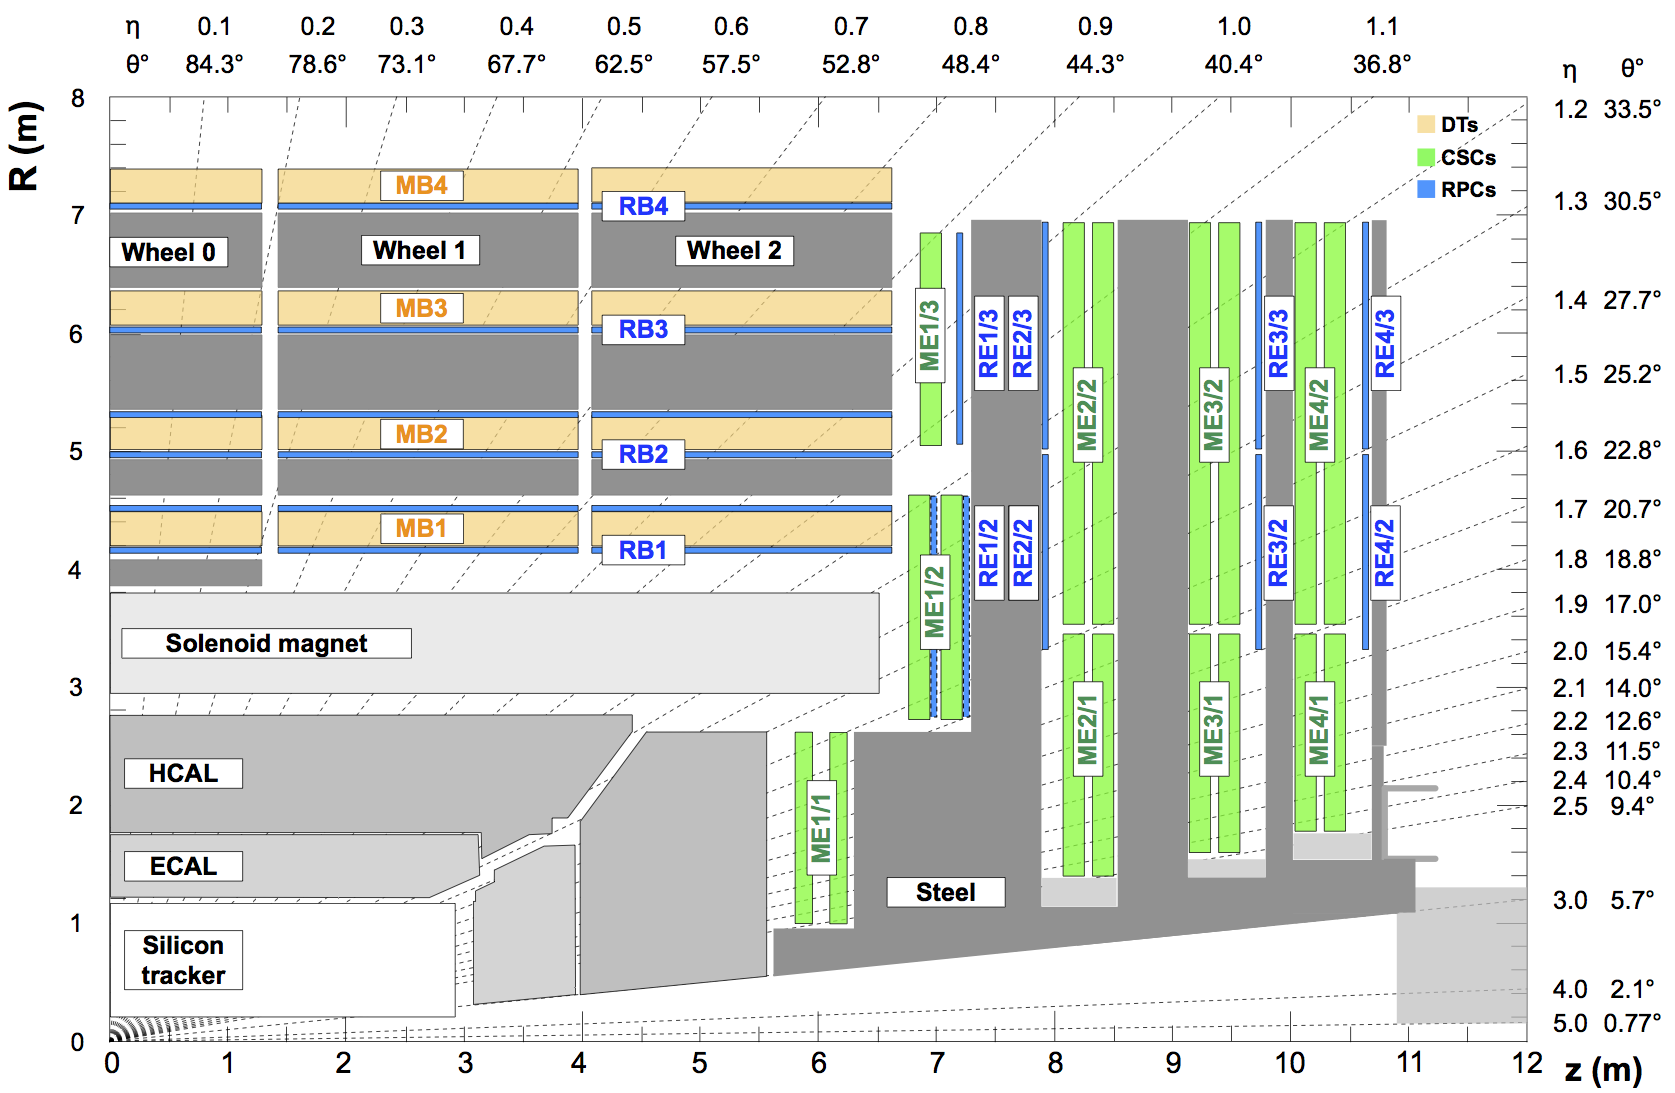
\includegraphics[width=\textwidth]{../ImmaginiTesi/CMSEtaView.png} 
  \end{minipage}
  \caption{Settore di CMS (sinistra), vista di CMS  nella variabile $\eta > 0$ (destra)}
  \label{fig:SectorEtaView}
\end{figure}


Spesso l'alto rate di eventi di background a seguito di processi di interazione ad alta luminosità in LHC cela fenomeni interessanti: in questo contesto la rivelazione di muoni a CMS è uno strumento fondamentale per studiare tali fenomeni \cite{TheMuonProject}. Il sistema muonico di CMS ha quindi tre funzioni: identificazione di muoni, misurazione del momento e funzione di trigger.


Come mostrato in figura \ref{fig:LHC-CMS} e \ref{fig:SectorEtaView} la regione di barrel è formata da cinque ruote (\textit{wheel}), ognuna composta da dodici settori (\textit{sector}) e a loro volta da quattro stazioni concentriche (\textit{station}) interspaziate da una struttura di ferro che permette il ritorno del flusso di campo magnetico generato dal solenoide: pertanto in queste regioni l'intensità di campo è circa 2T. Nella regione di barrel, dove gli eventi di background sono minimi, per la rivelazione di muoni vengono impiegati drift tube (DT), celle contenenti fili di acciaio inossidabile anodico disposte in modo adiacente una all'altra separate da barre di alluminio che fungono da catodo: anodo e catodo operano ad un voltaggio rispettivamente di +3600V e -1200V. Quando un muone attraversa un DT la distanza tra la sua traiettoria e il filo di acciaio viene misurata a partire dal tempo di drift degli elettroni ionizzati che vengono attratti dal campo elettrico generato dalla differenza di potenziale tra catodo e anodo \cite{MasterThesisNicLai}. \newline
In totale CMS contiene 250 DTs, disposti nella regione di barrel come in figura \ref{fig:SectorEtaView} ricoprendo la pseudorapidità nel range $|\eta| < 1.2$. \newline
Nelle regioni di endcap di CMS, dove il rate di muoni e livello di background è elevato ed il campo magnetico non uniforme, vengono impiegate CSCs che, grazie al loro design, permettono di ricavare precise informazioni spaziali e temporali sulle tracce di muoni nel range di pseudorapidità $0.9 < \eta < 2.4$. Le RPCs sono invece impiegate sia nella regione di barrel sia nella regione di endcap, e permettono una assegnazione definitiva del BX grazie al loro rapido tempo di risposta \cite{MasterThesisNicLai, cms2008cms}.


\subsection{Sistema di trigger}
\label{sec:SistemaDiTrigger}

Non è possibile gestire in tempo reale la mole di informazioni generata da 40 milioni collisioni al secondo, per questo CMS è dotato di un sistema di trigger implementato come primo passo nella selezione di eventi fisici al fine di ridurre il volume di dati, mantenendo però quelli interessanti. Il sistema di trigger si suddivide in due stadi: il \textit{Level 1 Trigger} (L1T) e l' \textit{High Level Trigger} (HLT), Figura \ref{fig:TriggerSystem}. 

Il Level 1 Trigger è implementato in hardware nel sistema di CMS sfruttando dispositivi programmabili come Field Programmable Gate Arrays (FPGA) e Lookup Table (LUTs) che, unendo informazioni del sistema muonico e del calorimetro, riducono il tasso di eventi da 40MHz a 100KHz. Il processo di analisi preliminare e selezione deve avvenire rapidamente, in un tempo limite di circa 4 $\mu$s, per permettere a tutti gli eventi di essere analizzati dal trigger; per questo il sistema di trigger L1 si articola a sua volta in tre processi di analisi preliminare: \textit{locale}, \textit{regionale} e \textit{globale} \cite{MasterThesisNicLai}.\newline
Come mostrato in Figura \ref{fig:TriggerSystem} sistema di trigger quindi raccoglie separatamente informazioni \textit{locali} dai calorimetri elettromagnetici e adronici (ECAL, HCAL) e dal sistema muonico (DTs, RPCs, CSCs), generando Trigger Primitives. Queste vengono combinate dai rispettivi \textit{trigger regionali} che effettuano una classifica degli eventi sulla base di parametri come energia, momento trasverso e qualità. Fino a 108 candidati muoni vengono trasmessi al \textit{trigger globale muonico}, GMT, mentre le informazioni del sistema di trigger calorimetrico seguono un percorso a sé stante. Infine 8 muoni sono inviati al Global Trigger.

\begin{figure}[t]
  \centering
  \begin{minipage}[b]{0.40\textwidth}
      \centering
      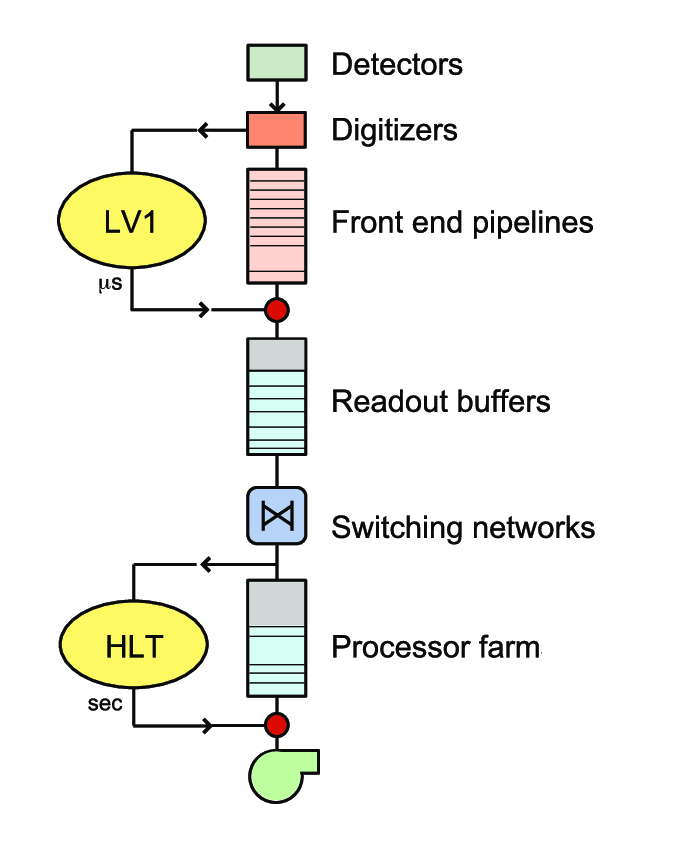
\includegraphics[width=\textwidth]{../ImmaginiTesi/TriggerSystem2.png} 
    \end{minipage}
    \hfill 
    \begin{minipage}[t]{0.58\textwidth}
      \centering
      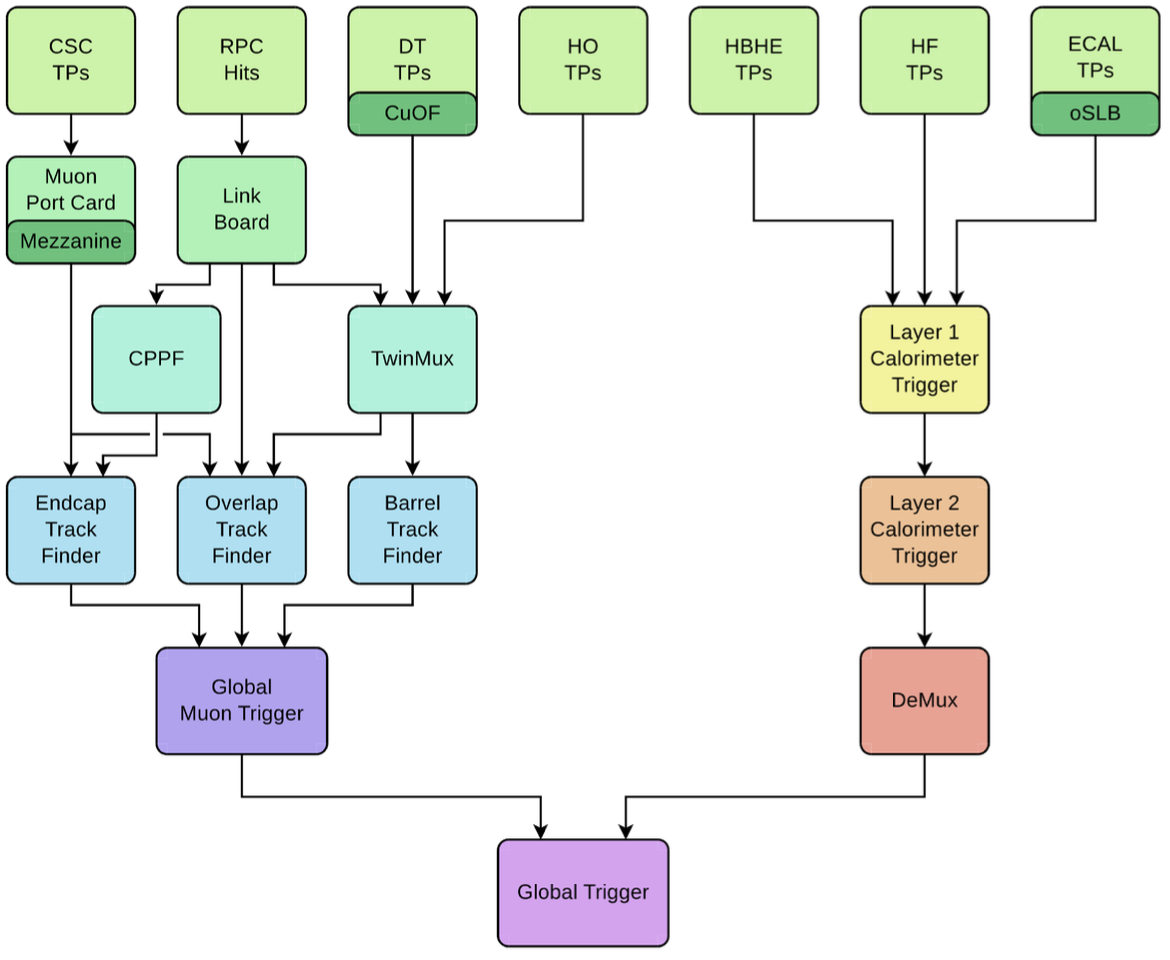
\includegraphics[width=\textwidth]{../ImmaginiTesi/TriggerSystemUpdate.png} 
  \end{minipage}
  \caption{Pipeline del sistema di trigger di CMS (sinistra), sistema L1T nel dettaglio (destra)}
  \label{fig:TriggerSystem}
\end{figure}

Studiamo ora più nel dettaglio il \textbf{sistema di Trigger Muonico}. Questo gioca un ruolo di fondamentale importanza nella la rilevazione e nel tracciamento di muoni nelle tre regioni delle camere muoniche che possono essere suddivise nei tre range in $\eta$ descritti in sezione \ref{sec:CMSDescrizione} al fine di migliorare l'efficienza di ricostruzione dei muoni. Di seguito è riportata una più dettagliata descrizione di questo sistema \cite{sirunyan2020performance}.\newline
Nella regione $1.2 < \eta < 2.4$ i segnali derivanti dai CSCs vengono usati dal sistema di tracciamento dell'endcap (\textit{Endcap Muon Track Finder}, EMTF) che, unendo le informazioni dei rilevatori, ricostruirà la traccia del candidato muone.\newline
Similmente nella regione $|\eta| < 1.2$, le Trigger Primitives (TP) provenienti dai detector DTs e RPCs della stessa stazione vengono processate dalle schede TwinMux, un sistema introdotto con la \textit{Phase 1} che permette, combinando le informazioni dei due detector, di ottenere una migliore risoluzione spaziale e temporale; i segnali combinati in uscita dal TwinMux sono chiamati \textit{superprimitives}, o stubs, ed ad ognuna viene assegnata una \textit{qualità}, che dipende dalle coordinate $\eta$ e $\phi$ delle TP in ingresso alle schede, e un \textit{angolo di curvatura interno} $\phi_b$. 
Si discuterà con maggiore dettaglio delle schede TwinMux nel Capitolo \ref{cap:SecondoCapitolo}. In base alla stazione e alla wheel in cui sono state generate le stubs, vengono inviate ai sistemi di tracciamento della regione di barrel (\textit{Barrel Muon Track Finder}, BMTF) o della regione di overlap (\textit{Overlap Muon Track Finder}, OMTF), o eventualmente entrambe, come mostrato in Figura \ref{fig:TriggerSystem}. Queste  ricostruiranno la traccia del muone usando le informazioni sull'angolo di curvatura $\phi_b$, ricavando anche informazioni riguardanti il momento trasverso $p_T$ del candidato muone. \newline
A questo punto fino a 108 tracce generate dai tre sistemi di tracking, corrispondenti a \textit{candidati muoni}, vengono inviate al Global Muon Trigger (GMT) che le classifica in base alla qualità, momento trasverso $p_T$ e provenienza (candidati muoni provenienti dalla regione di barrel possiedono infatti una qualità maggiore rispetto alla regione di endcap e overlap) e rimuovendo i duplicati. Infine 8 muoni vengono inviati al Global Trigger (GT). \newline
Infine il Global Trigger applica fino a 512 algoritmi di selezione sugli eventi ricevuti dal trigger muonico e da quello calorimetrico, decidendo se inviare un segnale di accettazione (Level 1 Accept) passando quindi l'evento all'HLT. La selezione applicata dal L1T permette di ridurre l'output di eventi da 40MHz a 100KHz \cite{CERNsummerSchool}.\newline
Gli eventi del GT che hanno ricevuto il segnale di accettazione, momentaneamente presenti nei buffer del Sistema di Front-End, vengono ulteriormente filtrati dal HLT che, al contrario del trigger L1, è implementato via software in una infrastruttura computazionale che conta 16000 CPU. \newline
Applicando complessi algoritmi di controllo qualità sui muoni del GT, l'HLT seleziona circa 1 evento su 100, riducendo quindi il rate di eventi da 100KHz a 1KHz \cite{MasterThesisNicLai}.


\section{La Phase 2 di CMS}
\label{sec:Phase2}

Come già accennato in Sezione \ref{sec:LHC}, a seguito della Run 3, nel 2026, verranno effettuati importanti aggiornamenti alle componenti di LHC, permettendo di raggiungere un picco di luminosità istantanea pari a $5 \times 10^{34}$ \Lumi. Di conseguenza CMS, ed in particolare il sistema di Trigger, deve essere a sua volta aggiornato per poter collezionare efficientemente il nuovo volume di informazioni di HL-LHC, che si stima raggiungerà, nella sua configurazione finale, circa 200 collisioni per Bunch Crossing. A CMS verranno implementati nuovi sensori che permetteranno di estendere la regione di raccolta dati fino a $|\eta| < 3.8$. Ulteriori miglioramenti verranno effettuati al sistema di trigger adronico, sostituendo l'elettronica dei calorimetri nella regione di barrel, ottenendo una risoluzione migliore oltre che informazioni temporali. \newline
Il sistema di Trigger muonico nelle regioni di barrel, overlap e endcap verrà modificato, sostituendo l'elettronica dei rilevatori con sistemi più moderni. I detector RPCs verranno migliorati (iRPC) e saranno installate delle camere GEM (Gas Electron Multiplier). \newline
Verrà inoltre aumentato il rate di output massimo di eventi del L1T fino a 750KHz e quello di HLT fino a 7.5KHz; verrà inoltre aumentata la latenza totale del L1T a 12.5 $\mu$s, permettendo per la prima volta di includere le informazioni dei calorimetri adronici \cite{collaboration2021phase}. Inoltre una maggiore latenza permetterà di implementare algoritmi più complessi per la ricostruzione e identificazione di oggetti usando tecniche di Machine Learning, oltre che nuovi algoritmi come \textit{Particle Flow Algorithm}. In Figura \ref{fig:Scouting} viene mostrato il nuovo sistema di Trigger Level 1 relativo alla Phase 2.

Inoltre gli upgrade relativi al Trigger L1 della Phase 2 non sono solo progettati per migliorare l'efficienza di selezione degli eventi rispetto alle performance attuali, ma anche per affinare significativamente la selezione di possibili eventi non predetti dal Modello Standard. Sfruttando la maggiore latenza del sistema di Trigger, si potranno inoltre applicare nuovi algoritmi specifici per la ricerca di eventi esotici.


\section{Data Scouting}
\label{sec:DataScouting}


\begin{figure}[t]
  \centering
  \begin{minipage}[b]{0.43\textwidth}
      \centering
      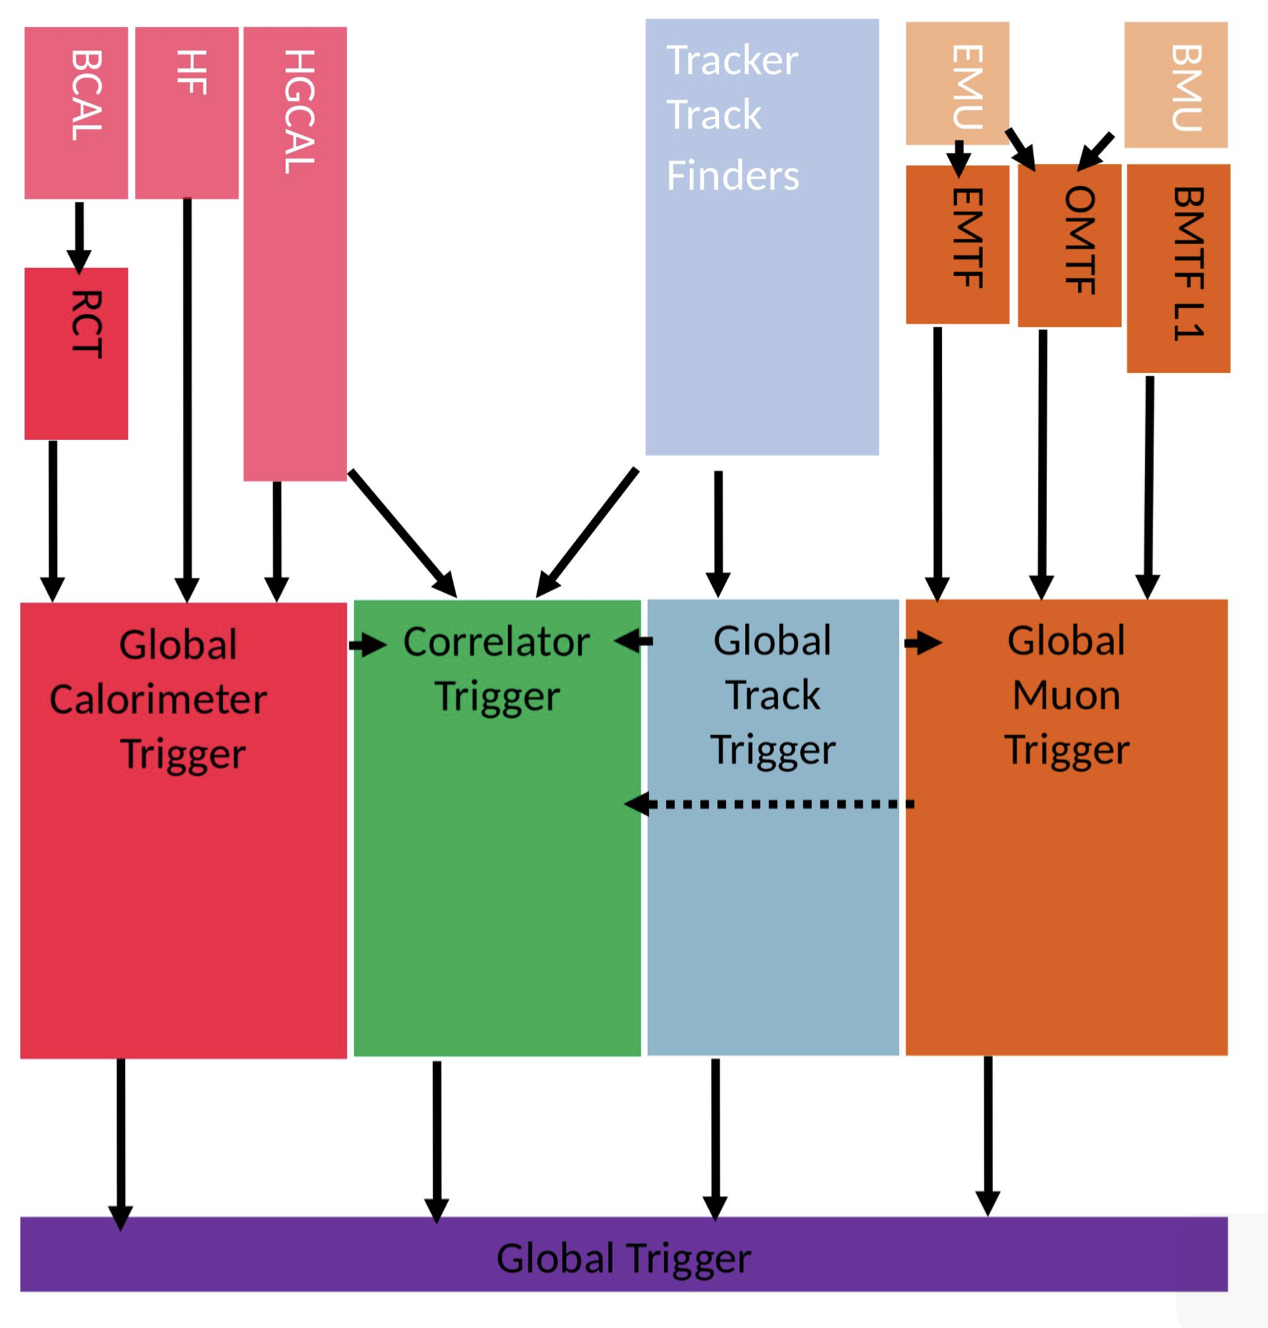
\includegraphics[width=\textwidth]{../ImmaginiTesi/Phase2.png} 
    \end{minipage}
    \hfill 
    \begin{minipage}[b]{0.48\textwidth}
      \centering
      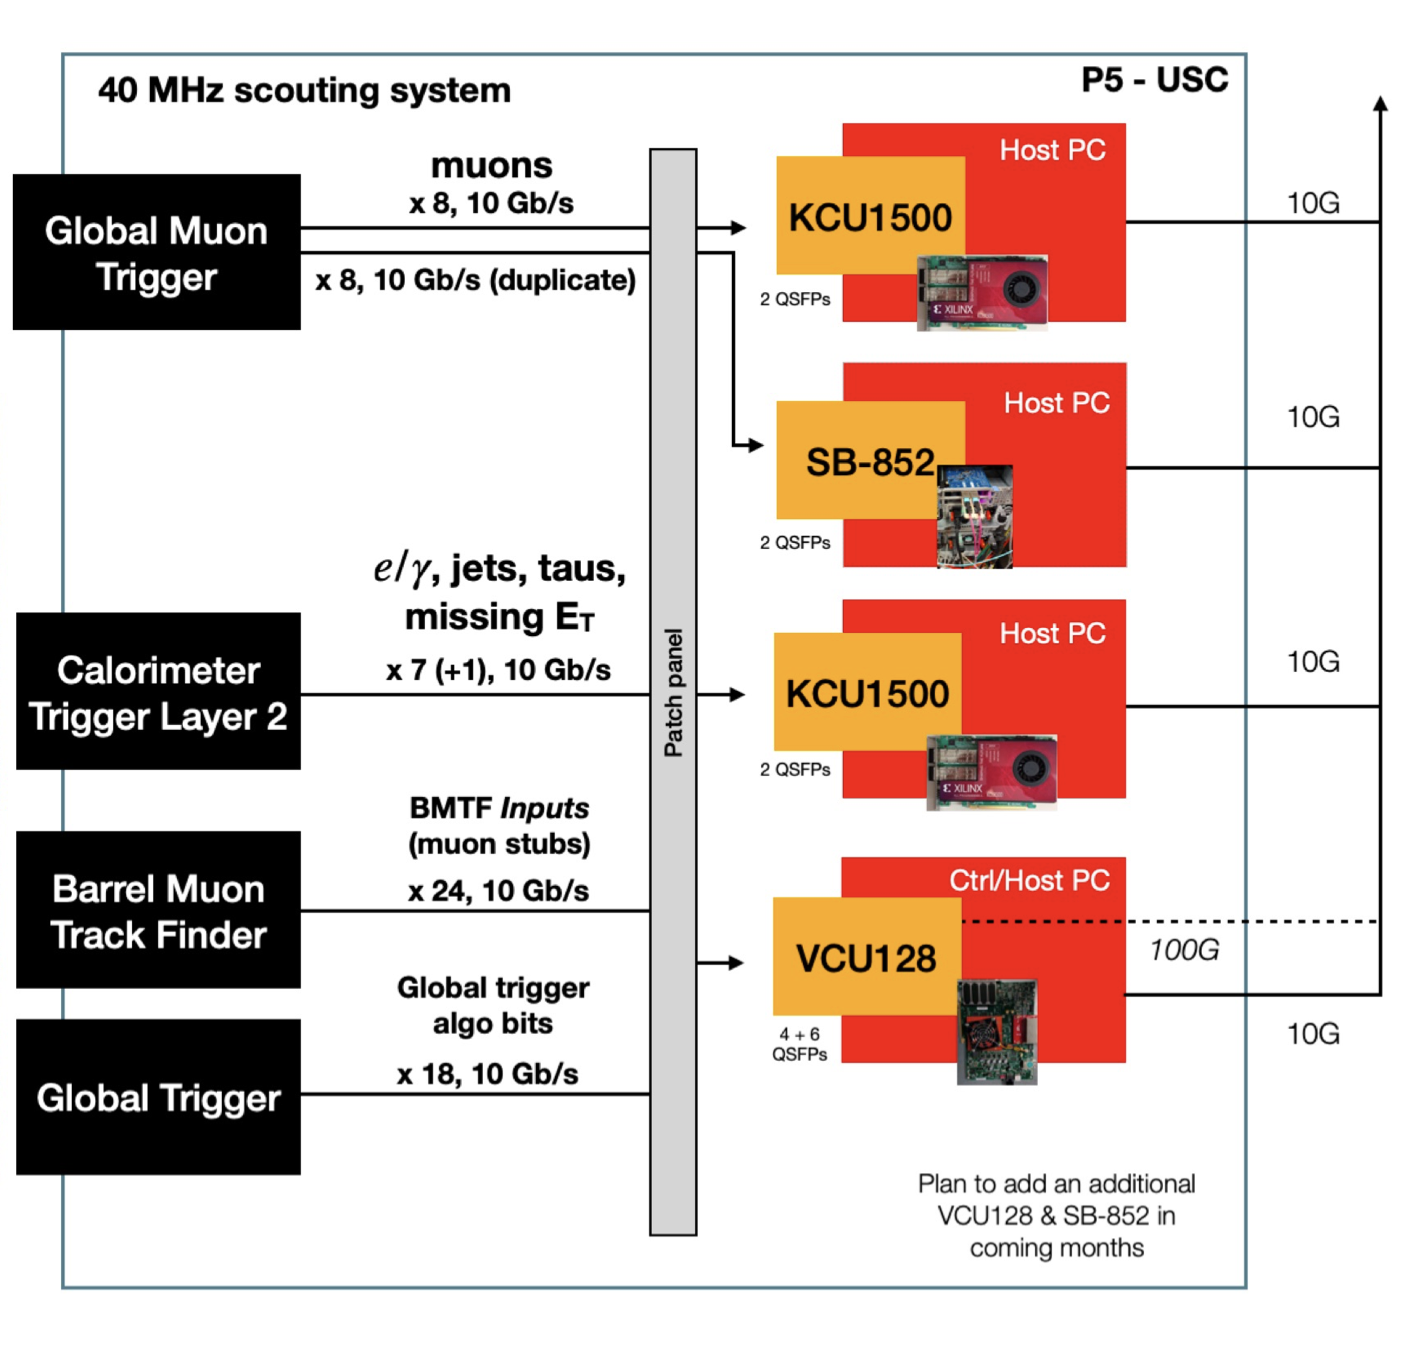
\includegraphics[width=\textwidth]{../ImmaginiTesi/DataScoutingRun3.png} 
  \end{minipage}
  \caption{Aggiornamento del sistema L1T di CMS a seguito della Phase 2 (sinistra), implementazione tecnica di Data Scouting nel L1T durante la Run 3 (destra)}
  \label{fig:Scouting}
\end{figure}

Lo scopo principale del sistema di Trigger di CMS è quello di selezionare una frazione degli eventi generati dalle collisioni protone protone, mantenendo solamente gli eventi di rilevanza secondo quanto detto in Sezione \ref{sec:SistemaDiTrigger}. Indubbiamente ciò introduce un \textit{pregiudizio} (bias) nella porzione di eventi minoritari che non vengono eliminati in quanto il sistema di Trigger filtra e seleziona dati che seguono leggi della fisica attualmente conosciute, possibilmente celando fenomeni sconosciuti e non teorizzati dal Modello Standard. \newline
In questo contesto il \textbf{Data Scouting} è un approccio che si basa sull'analisi degli eventi direttamente nella catena di Trigger, estraendo e processando online dati con una minore risoluzione, aggirando quindi il bias introdotto dal Trigger. \newline
La tecnica di Data Scouting è stata utilizzata per la prima volta a livello dell High Level Trigger dove, per costruzione, solo 1 evento su 400 viene accettato. Qui è infatti possibile introdurre una nuova pipeline parallela al percorso standard dell'HLT che effettui Data Scouting su oggetti fisici che verrebbero possibilmente rigettati dal Trigger.

Con l'introduzione della Phase 2 e dei miglioramenti al sistema di CMS, si è aperta la possibilità di eseguire Data Scouting a livello del L1T piuttosto che nell'HLT, permettendo quindi di analizzare online la totalità di eventi derivanti dalla collisione di protoni, ad un rate di 40MHz. In particolare ciò è possibile grazie all'introduzione del tracciatore nel L1T che, unito all'algoritmo Particle Flow, permette una ricostruzione di muoni più accurata, migliorando la risoluzione del momento trasverso dei muoni. Il nuovo sistema di Data Scouting funzionerà parallelamente e in modo indipendente dal sistema di Trigger usando le uscite ottiche supplementari delle schede di acquisizione del L1T, elaborando i dati usando sistemi computazionali esterni. Ciò permetterà di aggirare il bias introdotto dal sistema di Trigger, aprendo le porte ad uno studio più accurato di eventi non predetti dal Modello Standard \cite{MasterThesisNicLai}. Essendo inoltre il sistema di Data Scouting parallelo al sistema di Trigger, non deve soddisfare requisiti limite di latenza del sistema del L1T, ma deve comunque essere in grado di analizzare circa due milioni di eventi al secondo. Sono pertanto in sviluppo tecniche che sfruttano l'uso di Machine Learning, nello specifico \textit{reti neurali}, per migliorare l'efficienza di analisi del volume di dati raccolto \cite{MasterThesisNicLai}

Al fine di sperimentare l'utilizzo della tecnica di Data Scouting usando dati reali, durante la Run 3 un sistema apposito è stato implementato per raccogliere informazioni dai principali step di trigger del L1T. Più nel dettaglio il sistema raccoglie informazioni dal Barrel Muon Track Finder (BMTF), dal Calorimeter Trigger, dal Global Muon Trigger (GMT) e Global Trigger (GT) sfruttando una serie di schede FPGA diverse: in particolare, come mostrato in figura \ref{fig:Scouting} sono impiegate due schede \textit{Xilinx KCU1500}, una scheda \textit{Micron SB852} e una \textit{Xilinx VCU128}. \newline
I dati dal Global Muon Trigger e dal calorimetro vengono inviate alle schede Xilinx KCU1500 che hanno lo scopo di abbattere il rate di eventi di un fattore 10, eliminando i BX dove non sono rilevate tracce di muoni. Alla scheda Micron SB852 vengono inviati dei duplicati dei muoni del GMT: questa ha lo scopo di effettuare istogrammi istantanei per verificare la conformità delle misure di luminosità. Infine la scheda Xilinx VCU128 raccoglie le superprimitives in ingresso al BMTF e gli algoritmi usati dal GT, inviandole direttamente ad un PC commerciale.
